% Generated by tools/v11/build_floats.py; figure from tools/v11/build_effort_figure.py.
\begin{figure*}[t]
\centering
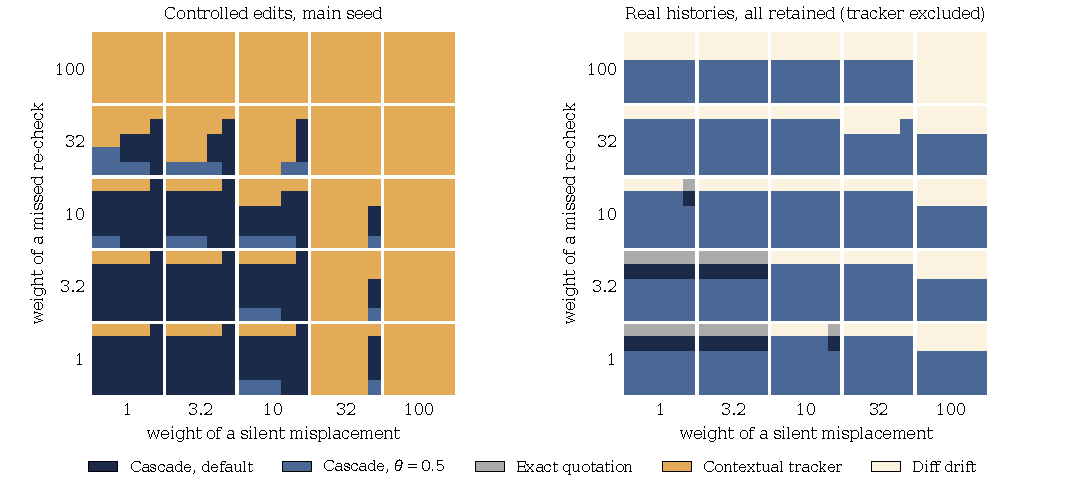
\includegraphics[width=\textwidth]{generated/effort-v11.pdf}
\caption{Cheapest method under the additive effort model. Weights are chosen values in units of the cost of one lost anchor; each outer cell fixes the weights of a silent misplacement (horizontal) and a missed re-check (vertical), and its inner grid varies the weights of an unnecessary re-check (horizontal) and of a wrong placement that requests re-check (vertical) over the same log-spaced grid. The real-history panel omits the contextual tracker, whose rates Table~\ref{tab:safety} reports, because its execution failures have no defined inspection cost; the evidence package reports that sensitivity separately.}\label{fig:effort}
\end{figure*}
